Abarcaré la posición de Jorge A. Sábato principalmente desde su artículo más conocido con Natalio Botana: \textit{La ciencia y
la tecnología en el desarrollo futuro de América Latina}.

En dicho artículo, los autores presentan un triángulo de relaciones (como el detallado en la Figura \ref{triangulo}) en el cual cada vértice
corresponde a un actor:
\begin{itemize}
    \item Gobierno: el conjunto de roles institucionales que tienen como objetivo formular políticas y movilizar recursos de y hacia los otros vértices a través de los procesos legislativo y administrativo.
    \item Infraestructura científico-tecnológica: el conjunto de sistemas educativos, institutos de investigación, academias de ciencias, etc.
    \item Estructura productiva: el conjunto de sectores productivos que provee los bienes y servicios que demanda una determinada sociedad.
\end{itemize}

\begin{figure}[H]
    \centering
    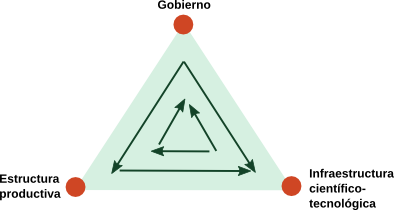
\includegraphics[width=0.6\textwidth]{imagenes/sabato.png}
    \caption{Triángulo de Sábato/Botana}\label{triangulo}
\end{figure}

% Luego, cada vertice tiene responsabilidades y se espera que se relacione con los demás de ciertas maneras.

En el artículo mencionado, Sábato habla de autonomía como la capacidad de decisión propia, y menciona que esta es el resultado de un proceso deliberado de interrelaciones entre los vértices.

Entonces, la postura de Sábato en cuanto a la relación entre autonomía tecnológica y
autonomía nacional se puede analizar desde las responsabilidades que plantea para los distintos vértices, junto con sus relaciones.
% Este proceso se establece a través del flujo de demandas que circulan en sentido vertical (gobierno - los otros dos vertices) y en sentido horizantal.

Sábato distingue tres tipos de relaciones posibles:

\begin{itemize}
    \item \textit{Intrarelaciones}: las que suceden entre los diferentes componentes de un mismo vértice.
    \item \textit{Interrelaciones}: las que suceden entre dos vértices de un mismo triángulo.
    \item \textit{Extrarelaciones}: las que suceden entre dos vértices de triángulos distintos.
\end{itemize}

De las \textbf{intrarelaciones}, basta mencionar que deben estructurarse con vista a garantizar una determinada \textit{capacidad} para generar, incorporar o transformar demandas en un producto final que es la innovación científico-tecnológica. En particular:

% Si hablamos de relaciones internas dentro de cada vertice, \textit{intrarelaciones}, éstas tienen por objetivo transformar a estos centros de convergencia
% en centros capaces de generar, incorporar y transformar demandas en un producto final que es la innovacion cientifico-tecnologica. Es decir:

\begin{enumerate}
    \item El vértice-gobierno requiere la capacidad para realizar una \textit{acción deliberada} en el ámbito de políticas científico-tecnológicas, con el fin de formular un cuerpo de doctrina, de principios y estrategias capaces de fijar metas posibles, cuyo logro depende de una serie de decisiones políticas, de la asignación de recursos y de la programación científico-tecnológica.
    \item El vértice-infraestructura científico-tecnológica requiere la \textit{capacidad creadora}: un científico mediocre producirá ideas mediocres, por más dinero que se les inyecte.
    \item El vértice-estructura productiva requiere \textit{capacidad empresarial}, publica o privada, que se puede definir según las ideas desarrolladas por Schumpeter, como aquella función que ``consiste en reformar o revolucionar el sistema de producción, explotando un invento o, de manera más general, una posibilidad técnica no experimentada para producir una mercancía nueva o una mercancía antigua por un método nuevo, para abrir una nueva fuente de previsión de materias primas o una nueva salida para los productos, para reorganizar una industria, etc''.
\end{enumerate}

El tercer ítem está fuertemente relacionado con las ideas de Bayer de que las políticas tecnológicas deben buscar explotar las potencialidades existentes.

% En este sentido, Sábato muestra estar de acuerdo con Bayer en que no sólo hay que lograr innovar en tecnología, sino que ademas ésta debe favorecer el desarrollo social y bienestar general.

\vspace{0.5em}

En cuanto a las \textbf{interrelaciones}, Sábato les asigna una responsabilidad mayúscula: la generación de una capacidad de decisión propia en el campo científico-tecnológico es el \textit{resultado de un proceso deliberado de interrelaciones} entre el vértice-gobierno, el vértice-infraestructura científico-tecnológica y el vértice-estructura productiva.
Es decir, que la conquista de la autonomía tecnológica depende \textit{fuertemente} de las interrelaciones que logremos construir entre los vértices del triángulo.

Además, Sábato señala que el vértice de la infraestructura científico-tecnológica depende vitalmente de la acción deliberada del gobierno, entendido en un sentido muy amplio, sobre todo en lo que se refiere a asignación de recursos. Sin embargo, el vértice-gobierno juega también el papel de centro impulsor de demandas hacia la infraestructura científico-tecnológica, y es aquí donde reside la dificultad mayor en el modo como se concebirá la formulación de programas una vez tomada la decisión política.

Esta idea concuerda con la posición de Bayer de que \textbf{debe existir una decisión política enmarcada en un proyecto de conquista de la autonomía nacional}. Es decir, que si el gobierno incrementa los recursos de los demás vértices, pero no hace demandas sobre estos, sólo se conseguirá crecimiento aislado, que no contribuirá a la conquista de la autonomía. También es fácil ver que si un gobierno hace demandas sobre los vértices, pero no les provee con los recursos suficientes para funcionar, entonces los resultados obtenidos serán acotados o pobres en su calidad.

\vspace{0.5em}

En cuanto a las \textbf{extrarelaciones}, Sábato afirma: en una sociedad donde funciona el triángulo de relaciones, las aperturas que se realicen hacia el exterior en materia de exportación de ciencia y tecnología original o de adaptación de tecnología importada, producen beneficios reales, ya sea a corto o largo plazo.

Muy distinto es cuando estas aperturas se realizan entre vértices aislados con un triángulo plenamente desarrollado. Este problema es muy característico de las sociedades latinoamericanas, y explica un sin fin de problemas, como por ejemplo el éxodo de talentos. Mientras en nuestras sociedades el científico se encuentra desvinculado y aislado frente al gobierno y a la estructura productiva, en el nuevo lugar de trabajo, al cual lo conduce su exilio cultural, está automáticamente amparado por instituciones o centros de investigación que, a su vez, se encuentran insertos en el sistema de relaciones planteado.

En este punto es interesante hacer notar otra similitud entre el pensamiento de Sábato y Bayer: la percepción de que se necesita un proyecto claro a nivel nacional que busque la autonomía, ya que la falta de este trae problemas graves que aumentan la dependencia.

\vspace{0.5em}

Habiendo dicho esto, Sábato afirma que en América Latina no existe un sistema de relaciones como el mencionado, ni tampoco hay conciencia acerca de la necesidad impostergable de establecerlo, por lo que hay una doble exigencia para las naciones en vías de desarrollo que busquen alcanzar su autonomía:
\begin{itemize}
    \item Crear una conciencia global para que nuestras sociedades asuman este problema en sus dimensiones reales.
    \item Actuar eficazmente sobre aquellos sectores en los cuales se podrían optimizar los recursos escasos en función del sistema de relaciones perseguido.
\end{itemize}

Además, Sábato reafirma: corresponde al sector gubernamental formular una política tendiente a \textit{acoplar} la infraestructura científico-tecnológica al proceso de producción, ya sea creando los centros que así lo permitan o relacionando los centros ya existentes.

\vspace{0.5em}

Por último, quisiera dar un ejemplo concreto que presenta Sábato en su artículo \textit{Empresas y fábricas de tecnología}, de la creación en 1971 de una empresa Argentina estatal que responde a necesidades de desarrollo existentes en ese momento, la \textit{Empresa Nacional de Investigación y Desarrollo Eléctrico S.A.} (\texttt{ENIDE}). Su objetivo fundamental estaba definido en su estatuto como ``Producir, distribuir, comprar, vender, exportar, importar e intercambiar conocimiento técnico-científico en el campo de la energía eléctrica y sus aplicaciones'', y su creación obedecía a diversas circunstancias:

\begin{itemize}
    \item La existencia de un mercado importante y en rápido crecimiento.
    \item En el campo de la energía eléctrica, la Argentina era neto importador de tecnología.
    \item Existía capacidad científico-tecnológica apta para la producción de tecnología eléctrica. La demanda interna era, sin embargo, muy escasa y de poca significación cualitativa.
    \item Por tratarse de un tipo de actividad que tenía poca tradición en el país, sobre cuya necesidad no existía aún conciencia clara y que requería capital de riesgo, sólo el Estado estaba en condiciones de ponerla en marcha.
\end{itemize}

% Notas Sábato:
% - no al colonialismo mental
% - pensar el desarrollo tecnologico como motor del desarrollo social y economico del país.
% - solo mediante ese manejo autonomo tecnologico podra una nacion comenzar a marchar
%     en la dirección que eventualmente le permitira disponer en cada caso de la tecnologia más ajustada
%     a sus propios objetivos, más respestuosa de su acervo cultural, más conveniente para sus propias
%     necesidades y más adecuadas a sus dotaciones de recursos y factores.
%
% - tecnologia nacional: manejar la tencologia como mas le convenga al país,
% - ¿Qué desarrollar y que comprar ? A veces conviene desarrollar primero, para luego importar en mejores condiciones.
% - La relacion entre politica tecnologica y economica, es determinante.
% - En particular, el uso del poder de compra del estado es el instrumento más importante
%
% - se va a alcanzar autonomia tecnologica: no como autonomia que reniega de la participacion de tecnologica extranjera,
%     sino como capacidad tecnologica autonoma, de generacion de tecnologia y de incorporacion de tecnologia estranjera a modo de configuracion de paquetes.
%     Lo contrario sería la desagregacion de paquetes tecnologicos, es decir: una participacion de componentes nacionales.
%
% - dependencia tecnologica: incorporación sumisa de las tecnologías disponibles por razones de disponibilidades y precios en el mercado.
% - autonomia: capacidad de desarrollo local: construir el triángulo, interrelacinando los tres vertices. Solo puede pasar si el estado tiene
%     una participacion clave en la estructura productiva.
% - presidente de SERBA: Empieza identificando cuales son los productos en los cuales puede haber desarrollo
%     tecnologico local y en los cuales podíamos prescindir de componentes importados.
% - Industrialización sustitutiva de importaciones.
% - Regimenes de promocion del desarrollo industrial, bastante protectivos: proteger a la industria naciente.
% - De vuelta: el compre nacional es un factor clave para la autonomia tecnologica, muestra una preferencia en cuanto proveedores externos.
% - Regulación de transferencia de tecnología extranjera
%
% -Por tanto, la desagregación tecnológica es también un instrumento de política industrial que busca maximizar
% la participación propia en la ejecución de proyectos de inversión por medio del incremento del componente tecnológico
%  nacional en la producción de un bien o de un servicio. Para eso es preciso investigar, en detalle, los agregados humanos,
%   económicos y técnicos de cada uno de los proyectos de inversión.

% http://www.fundacionsadosky.org.ar/seminario-ciencia-y-tecnologia-en-el-pensamiento-de-jorge-sabato-oscar-varsavsky-y-amilcar-herrera/
